\documentclass[14pt,a4paper]{extarticle}
\usepackage[utf8]{inputenc}
\usepackage[russian]{babel}
\usepackage[hyperref,hyperprint,spisok]{style/project}
\usepackage[left=3cm,right=1cm, top=2cm,bottom=2cm]{geometry}
%\usepackage{bbm}
%\usepackage{omega}
\pagestyle{plain}

\usepackage{pdfpages}

\renewcommand{\baselinestretch}{1.35}

\def\bm#1{#1}
\def\looser#1#2{#2}

\begin{document}
\includepdf[pages=2]{titul_prac.pdf}
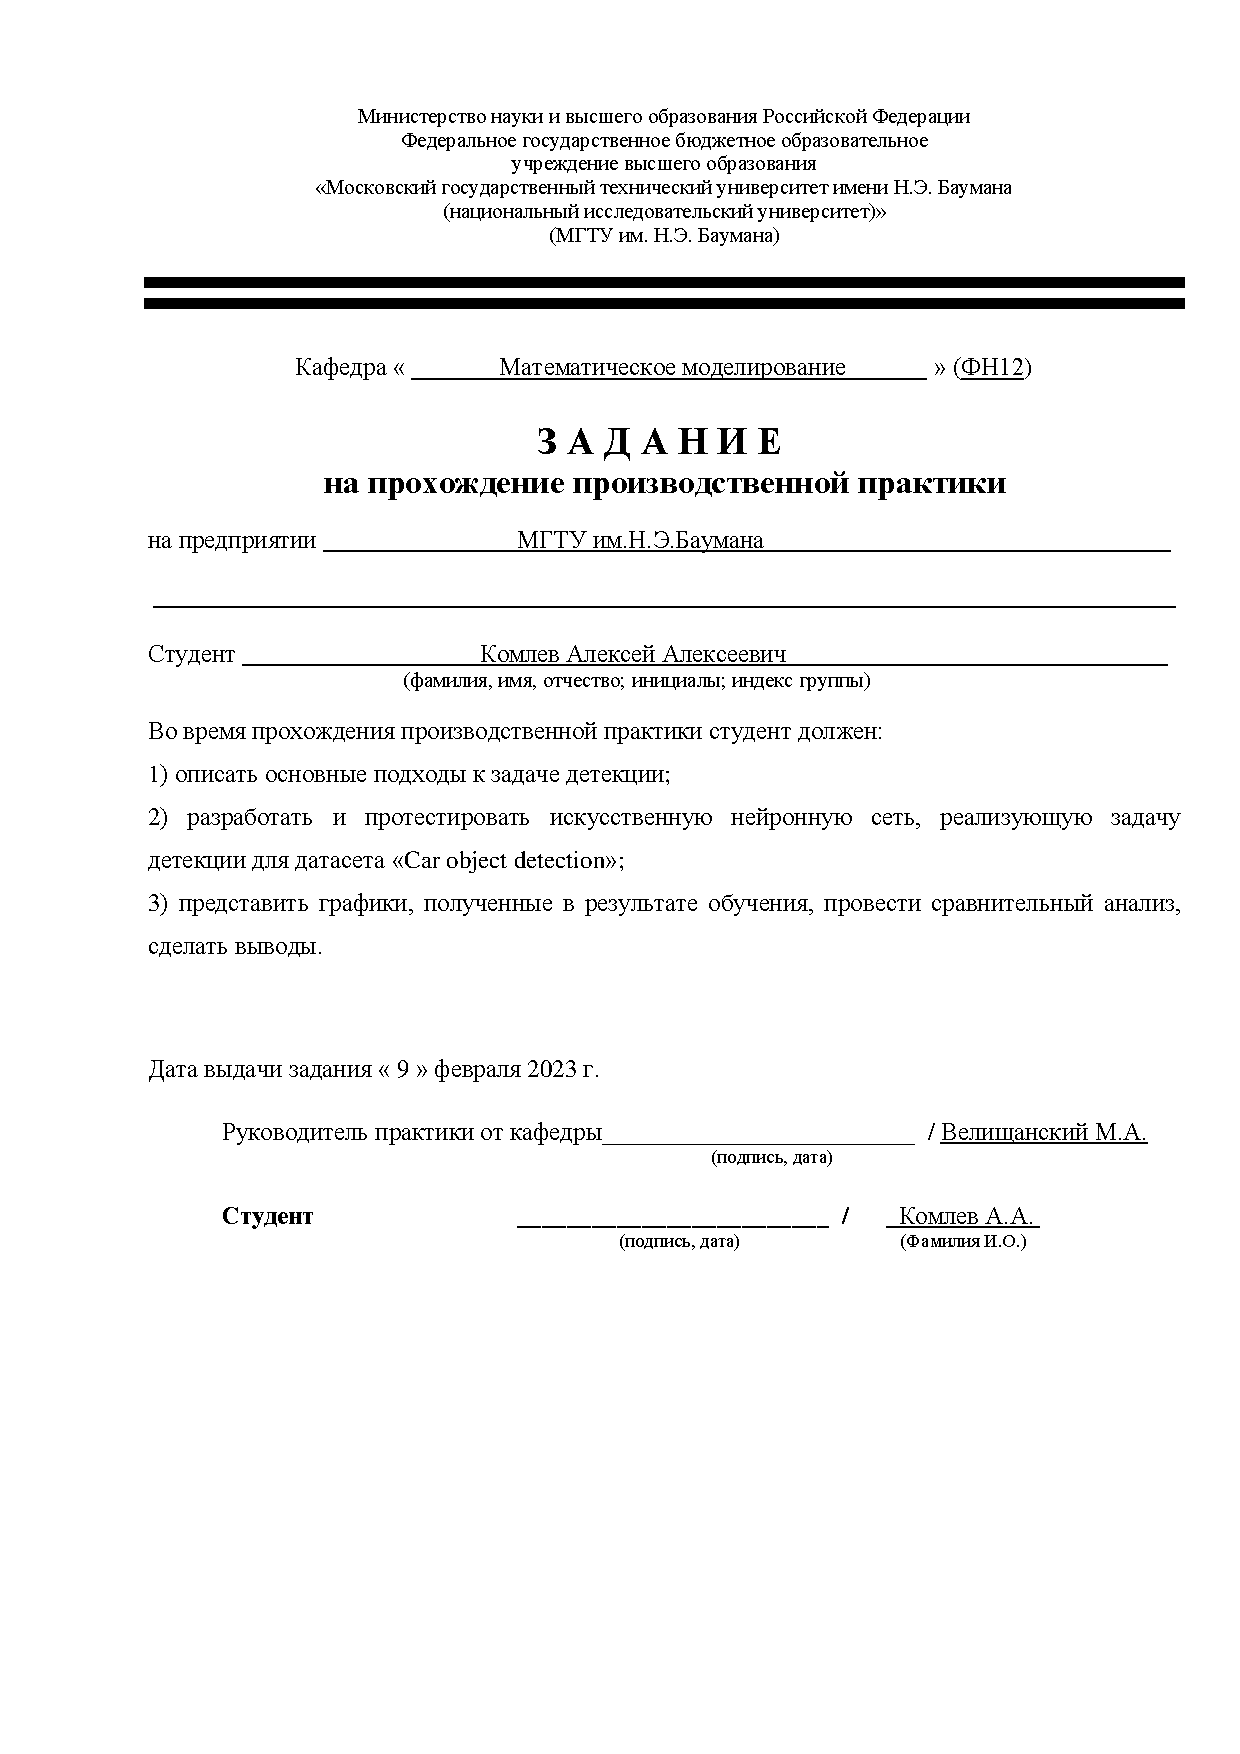
\includepdf[pages=1]{zadanie.pdf}

%\newpage

\tableofcontents

%\newpage


\section-{ВВЕДЕНИЕ}
Задача детекции изображений, связанная с выделением и классификацией объектов на изображении, является важной областью компьютерного зрения. 

Одним из ранних методов детекции является метод Виолы-Джонса, основанный на каскадных классификаторах, который был популярен в прошлом, но имеет некоторые недостатки, такие как невысокая точность обнаружения на изображениях в условиях изменения масштаба и поворота объектов.

Современные подходы для детекции объектов на изображениях основаны на использовании нейронных сетей.

R-CNN -- это первый метод детекции объектов на изображении, основанный на нейронных сетях. Он использует сверточные нейронные сети для извлечения признаков из областей изображения, а затем классифицирует и локализует объекты. Однако сеть R-CNN работает медленно из-за необходимости обрабатывать каждую область изображения отдельно.

Fast R-CNN -- улучшенная версия R-CNN, которая использует более эффективный способ обработки областей изображения с помощью RoI-pooling. Он также улучшает скорость и точность детекции объектов на изображении.

Faster R-CNN -- это метод, основанный на более эффективном процессе выделения областей изображения и RoI-pooling, называемом Region Proposal Network (RPN). Он может автоматически генерировать регионы интереса, что увеличивает скорость детекции.

С другой стороны, YOLO (You Only Look Once) -- это метод, который выделяет объекты и классифицирует их на изображении в один прогон. Он использует сеть, которая делит изображение на сетку ячеек, каждая из которых ответственна за предсказание объектов в этой ячейке.

SSD (Single Shot MultiBox Detector) -- похож на YOLO, это ещё один метод одноступенчатого обнаружения объектов, который предсказывает класс и ограничивающие рамки в одну попытку. Однако он использует другой подход к разделению изображения на набор якорных коробок с заранее определенными соотношениями сторон, масштабами и позициями.

Трансформеры -- это архитектура нейронных сетей, которая изначально была разработана для обработки текстов, но также может быть использована для обработки изображений с помощью <<механизма внимания>>. Использование трансформеров позволяет задействовать глобальный контекст изображения и агрегировать информацию из различных групп областей изображения. Примерами нейронных сетей, основанных на трансформерах, которые были успешно применены в задаче детекции объектов на изображении, являются DeTr и ViT.

DeTr -- это одна из первых нейронных сетей, полностью основанных на трансформерах. Она показала превосходство над другими методами детекции объектов на изображении и демонстрирует высокую точность обнаружения. 

ViT -- это нейронная сеть, которая была разработана для обработки изображений в виде сетки пикселей, и основана на трансформере. Она также показывает хорошую точность при решении задачи детекции объектов на изображениях.

\newpage
\section{ЗАДАЧА ДЕТЕКЦИИ ИЗОБРАЖЕНИЙ}
Популярная в области компьютерного зрения задача детекции заключается в нахождении на изображениях и видеозаписях различных объектов, а также локализации их местоположения. Преимущественно данная область ограничивается прямоугольником, допускающим определенную параметризацию -- изменение угла, ширины,высоты и т.д. В соответсвии с формой детектируемого объекта вместо прямоугольника может быть выбрана другая фигура, например, эллипс или окружность.

Формально задачу можно представить следующим образом:

1) пусть задан набор $s$ исследуемых классов, которым принадлежат объекты;

2) на вход подаются цветные (черно-белые) изображения $I \in R^{N \times M \times C}$;

3) требуется получить выходной набор обнаруженных объектов 
$$Obj = \{Obj_i | i = 1,..., p\},$$ 
где $Obj_i$ -- структура, которая описывает местоположение объекта (bounding box), а также класс $c_i \in [1, s]$, которому он принадлежит.  

Достоверность детекции зависит от нескольких факторов. Так, чтобы улучшить точность локализации, необходимо добавить угол поворота объекта. Описание границы объекта или области может способствовать более точному описанию его положения. 

Детектируемых объеты могут быть условно разделены на две группы. К первой категории относятся объекты, обнаружение которых может быть ограничено прямоугольником -- люди, животные, материальные предметы и т.д. Вторую группу образовывают <<неисчисляемые>> материалы, которые не имеют конкретной формы, размера, а их описание задано какой-либо текстурой -- вода, небо, земля и т.д.

Ограничивающая рамка может быть задана с использованием четырех пространственных координат в двух видах:

1) классический формат -- задание координат $(x_{min}, y_{max})$ левого верхнего и координат $(x_{max}, y_{min})$ правого нижнего углов;

2) центрированное задание -- определение координат центра $(c_x, c_y)$ прямоугольника, а также высоты $h$ и ширины $w$. 

В настоящее время задача обнаружения объектов является довольно час\-той в сфере автотранспортного движения в связи с развивающимися технологиями беспилотного управления и контроля трафика. Большое число существующих методов требует изучения их применения и усовершенствования для реализации задач детектирования в режиме реального времени. 

\newpage
\section{ПОДХОДЫ К ЗАДАЧЕ ДЕТЕКТИРОВАНИЯ}
Наиболее популярным направлением в области распознавания и детектирования объектов являются искусственные нейронные сети. В тех случаях, когда заранее известны возможные типы объектов, хорошее качество решения задачи показывают алгоритмы, использующие сверточные нейронные сети (CNN). Использование подобного семейства сетей позволяет обнаружать объекты разных классов и пространственных размеров. 

Можно выделить два основных подхода применения CNN:

1) ряд задач может быть реализован посредством применения готовых или уже предобученных архитектур; они могут детектировать объекты, на которых производилось обучение;

2) для других более частных задач может быть применена новая база изображений с целью дообучения модели, для которой имеется предобученная архитектура, в соответствии с поставленной задачей; данных случай предполгает настройку весов, в основном, исключительно для последних полносвязных слоев. 

Изучение и развитие детекторов (алгоритмов, позволяющих выделять объекты), а также хорошие показатели качества их работы привело к возникновению большого разнообразия нейросетевых архитектур. 

\subsection{Метод скользящего окна}
Первым, однако наиболее затратным с точки зрения вычислений, считается метод скользящего окна. При таком подходе происходит пошаговый проход по всему изображению, во время которого происходит извлечение определенного региона, а также классифицирование объекта, попавшего в него. 

Можно предположить, что простым вариантом послужит построение модели обнаружения объектов на основе модели, реализующей классификацию. Имея классификатор, который показывает хорошие результаты, можно обнаружать объекты, сдвигая <<окно>> по изображению и определяя, относится ли часть, ограниченная окном, к желаемому классу. Однако такой подход  ограничивается двумя проблемами:

1) какой размер окна считать оптимальным, чтобы объект точно содержался в нем; даже однотипные объекты (к примеру, теннисный мяч, футбольный мяч, относящиеся к классу мяч) могут иметь сильно отличащиеся пространственные размеры;

2) соотношение сторон ограничивающего прямоугольника -- сильно отличающиеся по форме объекты могут иметь разные пропорции сторон.

Решение описанных проблем требовало бы перебора различных скользящих окон, отличающихся размерами и формой. Это приводит к значительным вычислительным затратам.
 
\subsection{Метод предложения регионов}
Другим подходом в задаче детектирования является метод <<предложений регионов>> (region proposals), сочетающий в себе два алгоритма. Первый из них создает множество предположений -- это регионы, в которых может находиться объект. Второй алгоритм производит классифицирование объекта.  

Данный метод предполагает сначала нахождение некоторых областей на изображении, а заем объединение их в группу, согласно определенной иерархии. Такие области впоследствии объединяются согласно различным цветовым пространствам, а также факторам схожести. В результате имеется несколько предложений регионов, в которых может быть обнаружен объект за счет слияния нескольких небольших регионов.

Главным направлением развития глубоких нейронных сетей стало обнаружение объектов в реальном времени. Здесь можно отметить сеть R-CNN (Region Based). Данный подход характеризуется разпознаванием не по всему входному изображению, а в локализованной области. Основные шаги в реализации детектирования с использованием R-CNN моделей \cite{cnn}:

1) генерация областей интереса для входного изображения -- предложение регионов, которые предположительно могут содержать объект;

2) формирования карты признаков -- происходит масштабирование сгенерированных на предыдущем этапе областей до размеров, соответствующих архитектуре нейронной сети CNN, эти данные поступают на вход CNN;

3) классификация -- каждый объект определяется к своему классу посредством применения полученного вектора признаков с использованием метода опорных векторов.

Прежде чем осуществить классификацию для каждого предложенного региона используется алгоритм подавления немаксимумов. Его суть заключается в том, что исключительно локальные максимумы могут быть рассмотрены в качестве контура объекта. Применение такого алгоритма обусловлено необходимостью избавления от дублирующих областей на входном изображении.

Оценка качества произведенной классификации производится с помощью часто применяемой в задачах компьютерного зрения метрики Intersection over Union (IoU). Данное значение равняется отношению площади пересечения прямоугольника (области интереса), который был получен в ходе обнаружения, и  прямоугольника из разметки к площади их объединения:
\begin{equation}
IoU = \dfrac{B_1 \cup B_2}{B_1 \cup B_2}.
\end{equation}

Среди минусов использования R-CNN сетей можно отметить их относительно медленную работу, а также то, что в ходе алгоритма рассматриваются лишь отдельные области, а не изображение в целом.

\subsection{Детекция за один проход}
Еще одну группу методов детекции составляют такие, в которых локализация и классификация осуществляются одновременно, то есть алгоритм проходит один раз. Данный подход получил название <<Single Shot Detection>> (SSD, <<детекция за один проход>>). 

SSD-алгоритм представляет собой комбинацию двух компонентов -- базовой модели и <<головы>>. Первая модель, базовая, является сетью для классификации (средством для извлечения признаков на изображении), которая была предварительно обучена. Преимущественно ею является сеть наподобие ResNet, обученная на ImageNet. При этом из данной сети удален последний полносвязный слой. В результате имеется глубокая нейронная сеть, умеющая находить семантическое значение для изображения, поступающего на вход, для которого сохранена пространственная структура, несмотря на более низкое разрешение. 

Головная часть SSD задается одним или несколькими слоями, добавленными к базовой модели. Данные выхода могут быть интерпретированы как ограничивающие прямоугольники и классы объектов в пространственном расположении активаций конечных слоев. Архитектура сверточной нейронной сети с SSD-детектером схематично представлена на рис. \ref{ssd_fig_lbl}.
\begin{figure}[h]
\center{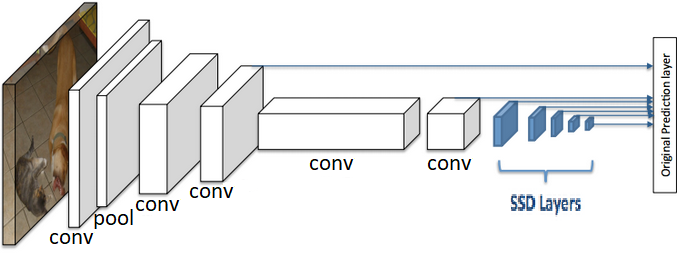
\includegraphics[width=1.0\linewidth, height=0.4
\textheight]{data/ssd_fig}}
\caption{Сеть с SSD-детектером}
\label{ssd_fig_lbl}
\end{figure}  

Белые прямоугольники на рис. \ref{ssd_fig_lbl} соответствуют базовой модели, а последние слои, представленные синими прямоугольниками, отвечают голове SSD. 

В отличие от метода скользящего окна, SSD-алгоритм использует разделение изображения на сетку, каждая ячека которой производит нахождение объектов в свооей области. В случае отсутствия объекта он рассматривается в качестве фонового класса, а его местоположение игнорируется. Расположение и форма объекта выводится самостоятельно каждой ячейкой. 

Для случая, когда в одной ячейке могут содержаться сразу несколько объектов, вводятся такие понятия, как якорная рамка (фиксированная рамка) и рецептивное поле.

1. \textbf{Якорная рамка (anchor box).} Каждой клетке сетки может соответствовать несколько якорных/приоритетных рамок. Метод SSD опирается на фазу сопоставления в процессе обучения. По сути происходит предсказание класса детектируемого объекта и его местоположения. На практике каждый якорный блок определяется соотношением сторон и уровнем масштабирования. 

Описываемая архитектура позволяет учесть, что форма предметов необязательно может быть квадратной, за счет предварительно заданных соотношений сторон для anchor box. Размер якорной рамки необязательно должен совпадать с размером ячейки сетки. С этой целью вводится параметр zooms -- значение, определяющиее, насколько должны увеличиваться или уменьшаться рамки по отношению к каждой ячейке сетки. 

2. \textbf{Рецептивное поле.} Рецептивным полем называется такая область входного пространства, на которую воздействует конкретная функция CNN. Оно является главной предпосылкой SSD-архитектур, поскольку позволяет обнаруживать объекты разных масштабов, а также определять более узкую рамку. 

Говоря о методах, позволяющих обнаружать объекты в один прогон, следует также упомянуть алгоритм YOLO (You Only Look Once). 

\newpage
\section{НЕЙРОСЕТЕВЫЕ АРХИТЕКТУРЫ В ДЕТЕКТИРОВАНИИ}
\subsection{Архитектура Transformer}
Большое разнообразие нейросетевых архитектур для решения задач компьютерного зрения позволяет находить наилучшие комбинации, которые улучшают точность алгоритмов и скорость их работы. Одним из таких инструментов стала архитектура Transformer-моделей. 

Изначально данный агоритм использовался для решения задач обработки естественного языка. Однако модель трансформера оказалась довольно универсальной и масштабируемой, что позволило использовать ее и для других проблем глубокого обучения.

Предпосылкой создания такой архитектуры стало несовершенство использования рекуррентных нейронных сетей (RNN), котрые являлись основным методом работы с последовательностями. Среди их минусов можно выделить проблемы, описанные ниже.

1. В RNN-сетях информация о последовательности находится в закрытом состоянии. При этом обновление такого состояние происходит с каждым новым шагом. При необходимости модели вернуться к той информации, которая была получена многими шагами ранее, данные должны быть сохранены внутри самого скрытого состояния без изменений. Это приводит к необходимости выбора: либо хранить большой объем информации для скрытого состояния, либо отказаться от ее хранения совсем, следовательно, потерять эти данные.

2. Обучение RNN-сетей трудно поддается процессу распараллеливания. Это связано с тем, что для получения скрытого состояния на $i + 1$-ом шаге возникает необходимость получения состояния на $i$-ом шаге. В результате для батча примеров длиной в 1000 обработка будет составлять 1000 последоватлеьных действий. Такая процедура занимает довольно много времени, а также демонстрирует низкую эффективность при работе на GPU, которые используются при параллельных вычислениях. 

Таким образом, описанные проблемы осложняют использование рекуррентных сетей для дейчтвительно длинных последовательностей. Требуется подход, который мог бы считывать последовательность таким образом, чтобы вернуться к любому прошедшему моменту можно было за определенное время, сохранив исходную информацию. Этим свойством обладает структура self-attention (<<внимание к себе>>), которая лежит в основе архитектуры Transformer. 

Большая часть моделей, используемых для преобразования последовательностей, имееют структуру кодер-декодер \cite{cod_decod}. Здесь кодировщик отвечает за отображений входной последовательности представлений символов $(x_1, ..., x_n)$ в последовательность непрерывных представлений $z = (z_1,...,z_n)$. С учетом $z$ декодер затем генерирует вывод
последовательности $(y_1, ..., y_m)$ символов по одному элементу за раз. 
Transformer следует этой общей архитектуре. Общая схема сети Transformer представлена на рис. \ref{trans_arh_lbl}.
\begin{figure}[h]
\center{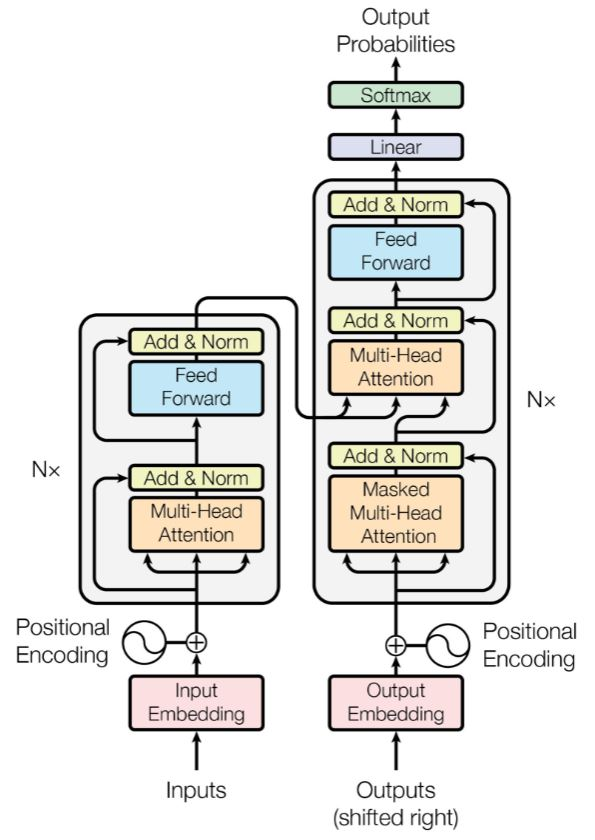
\includegraphics[width=0.6\linewidth]{data/trans_arh.jpg}}
\caption{Архитектура Transformer-сети}
\label{trans_arh_lbl}
\end{figure}  

Левая часть схемы представляет собой структуру энкодера. Он является стеком из идентичных слоев, каждый из которых имеет два подслоя \cite{transform}. Первый из них --  multi-head self-attention (<<механизм самоконтроля с несколькими головами>>). Второй -- это простая позиционная полносвязная нейронная сеть прямого распространения. После прохождения каждого из этих слоев выход и вход складываются (такой подход получил название residual connection), а затем следует слой layer normalization (блок <<Add \& Norm>> на рис. \ref{trans_arh_lbl}).

Декодерная часть также представляется несколькими слоями. В дополнение к двум
подуровням в каждом слое кодера, декодер вставляет третий подуровень, в котором используются выходы энкодера. Аналогично кодирующей части, происходит использование остаточных соединений
для каждого из подслоев с последующей нормализацией слоя. 

Проведем более детальный разбор основных составляющих архитектуры Transformer.

\textbf{Слой внимания.} Как было сказано выше, в сети трансформера используется слой self-attention. Данный слой отличается от обычного внимания тем, что на выходе получаются другие представления элементов последовательности, которая была подана изначально. При этом происходим взаимодействие элементов между собой.

Более детально, при вычислении внимания используется обучение трех матриц $W_Q, W_K, W_V$.Происходит умножение каждой из этих матриц на представление $x_i$ для каждого элемента последовательности на входе. При этом получаются вектора $q_i, k_i, v_i$, где $i$ соответствует номеру элемента, причем 

1) $q_i$ является запросом к базе данных;

2) $k_i$ -- это ключи, хранящиеся в базе; по ним будет происходить поиск;

3) $v_i$ отвечает самим значениям.

Понять, насколько близко значение ключа к запросу можно с использованием соотношения \ref{eq1}:
\begin{equation}
self-attention-weights_i = softmax\left(\dfrac{q_i k_1 T}{C}, \dfrac{q_i k_2 T}{C}, ... \right), \label{eq1}
\end{equation} 
где $C$ -- нормировочное константное значение. При этом в качестве $C$ может быть выбран квадратный корень $\sqrt{d_k}$ из размерности ключей и значений. 

Суммирование $v_i$ с новыми полученными коэффициентами являются выходом для $self-attention$-слоя. В матричном виде это можно представить выражением \ref{eq2}: 
\begin{equation}
self-attention(Q, K, V) = softmax\left(\dfrac{QK^T}{\sqrt{d_k}} \right)V.\label{eq2}
\end{equation}

\textbf{Слой Multi-head attention.} Конкретный набор значений $Q, K, V$ отовечает конкретному виду соотношений для токенов, данные матрицы получают при этом ограниченных набор данных из входных. Решением данной проблемы стал multi-head-attention подход, который заключается в том, что один слой внимания заменяется сразу несколькими параллельными, в каждом из которых используются свои веса. После этого результаты объединяются. Схематично данный слой представлен на рис. \ref{mul_head_lbl}.
\begin{figure}[h]
\center{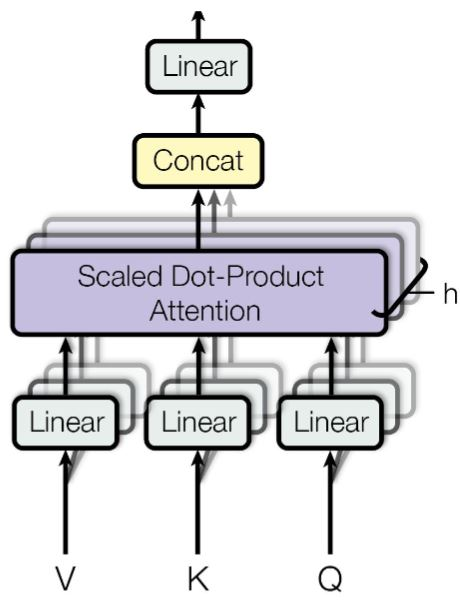
\includegraphics[width=0.45\linewidth]{data/mul_head}}
\caption{Слой multi-head attention}
\label{mul_head_lbl}
\end{figure}  


\textbf{Полносвязный слой.} Следующая часть блока сети Transformer -- полносвязная нейронная сеть прямого распространения (feed-forward network, FFN). Она включает в себя два полносвязных слоя, каждый из которых может независимо применяться к любому элементу для последовательности входа. В последнее время для архитектур выходное значение после прохождения первого слоя (промежуточное значение) может превышать выходы для блока в четыре раза. В связи с этим следует учесть, что для больших моделей FFN может работать значительно дольше, чем self-attention. 


\subsubsection*{Сеть Vision transformer}
Одним из наиболее значимых примеров того, где нашли применение Trans\-for\-mer-модели, стало компьютерное зрение. Архитектура, называемая Vision trans\-for\-mer, в свое время продемонстрировала наилучшие результаты в плане качества для задач классификации изображений. Этому поспособствовала реализация self-attention-идеи для изображений, которые были разделены на множество квадратных сегментов. В данном подходе изображения представляются в виде визуальных токенов, после чего подаются на вход сети. 

Общий алгоритм работы сети для решения задач компьютерного зрения представляется следующим образом:

1) получение карты признаков (feature map) для исходного изображения;

2) конвертация карт признаков в визуальные токены;

3) подача токенов на вход сети трансформера.

Выход сети может быть использван для решения задач классификации. В том случае, если объеденить выход с картой признаков, то может быть реализована задача сегментации. 

Архитектура Vision transformer (ViT) представляет собой комбинацию трех частей -- токенизатора, трансформера и проектора. 

Первый компонент, токенизатор, как следует из названия, отвечает за извлечение токенов. Второй осуществляет прохождение через сеть, которая была описана ранее, а третий производит сложение feature map и выхода трансформера. Схема ViT представлена на рис. \ref{vitr_lbl}.
\begin{figure}[h!]
\center{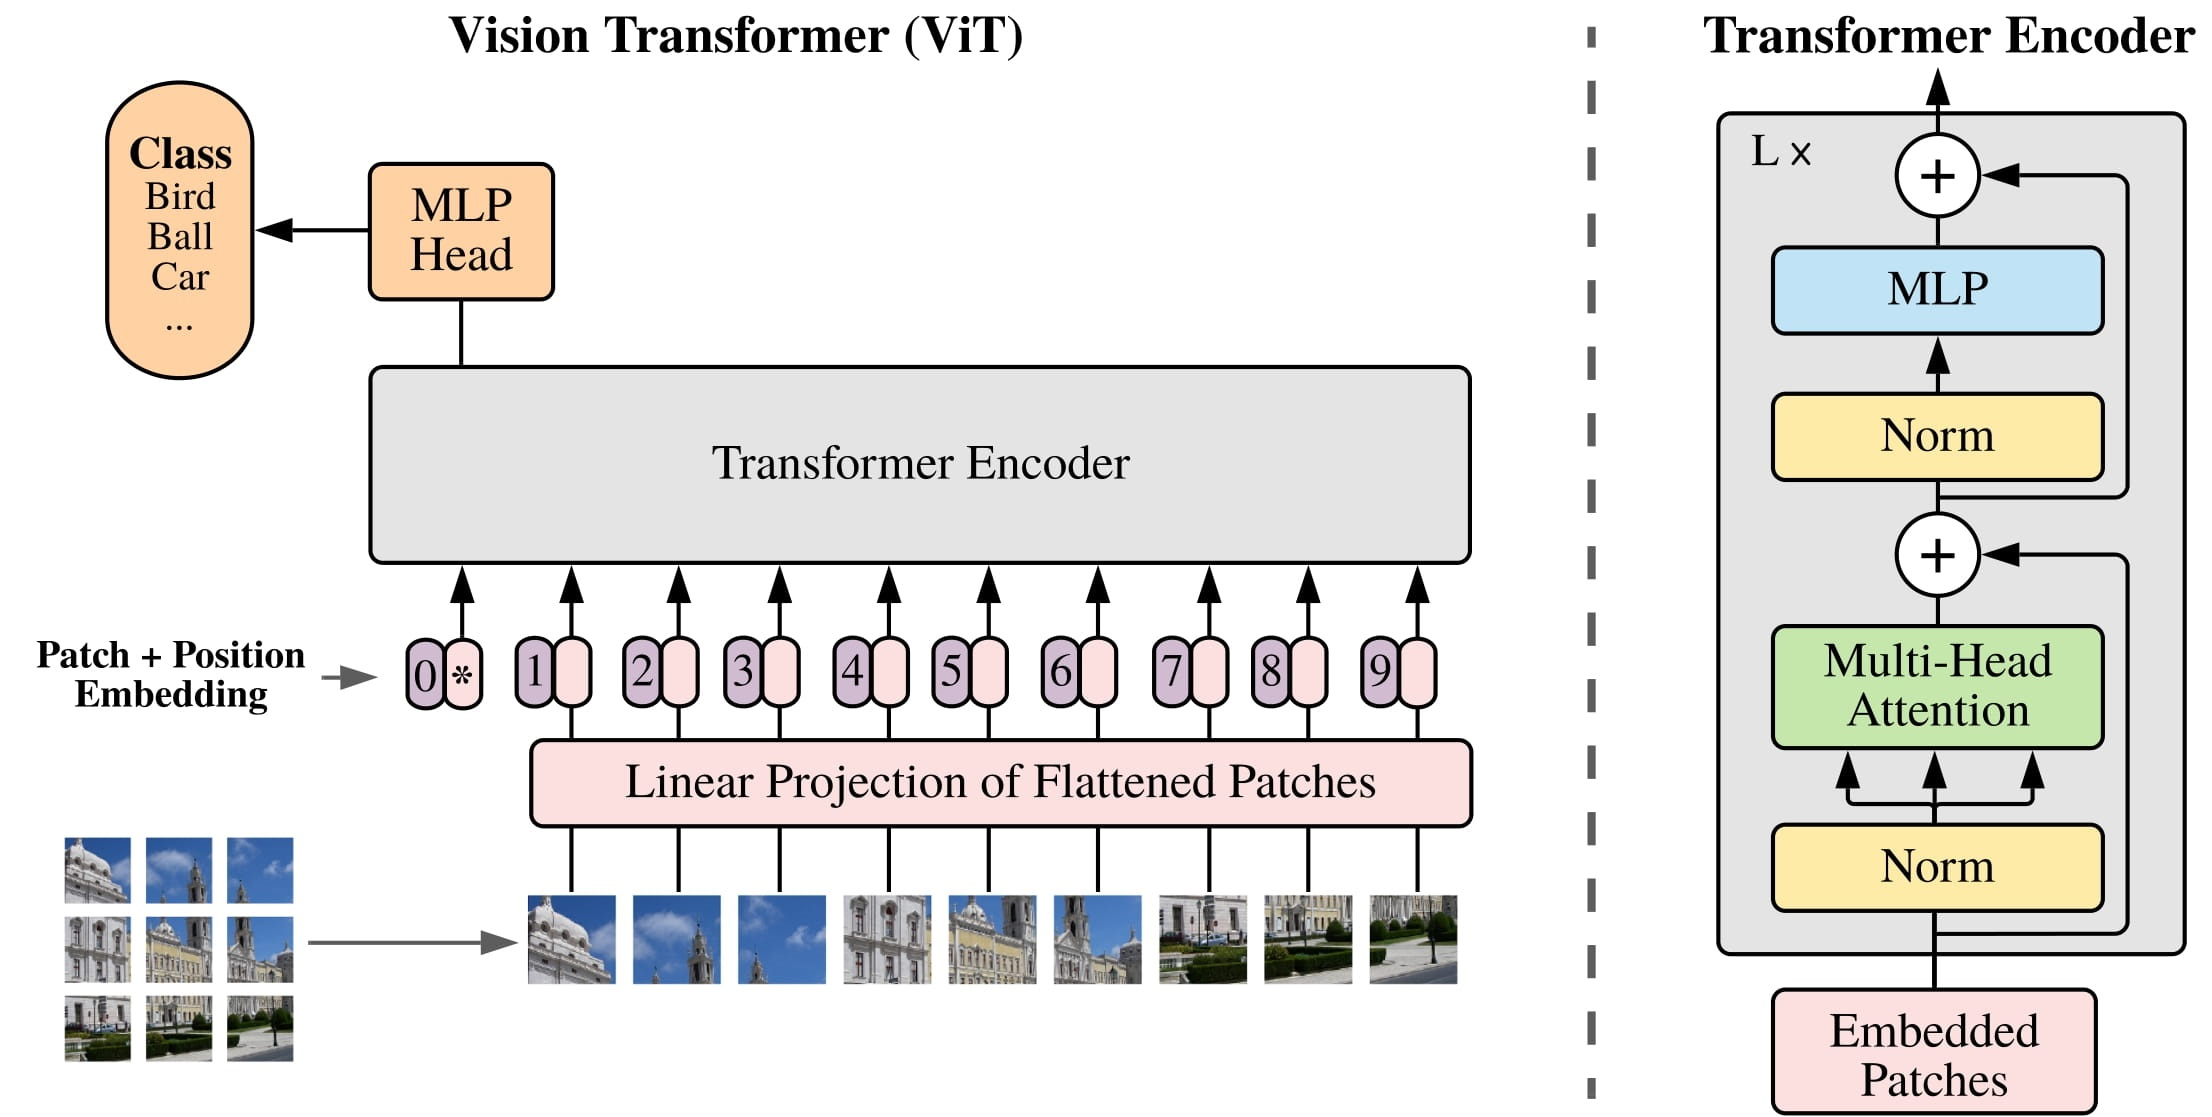
\includegraphics[width=0.95\linewidth]{data/vitr}}
\caption{Схема сети ViT}
\label{vitr_lbl}
\end{figure} 

\newpage
\subsubsection*{Сеть DETR}
Еще одной модификацией, которая используется для детектирования, является применение сети DETR (Object Detection with Transformers). В этом случае так же, как и для сети ViT, трансформер применяется не к самому изображению, а к признакам, которые были выделены сверточной сетью. Схема работы для сети DETR представлена на рис. \ref{detr_lbl}.
\begin{figure}[b!]
\center{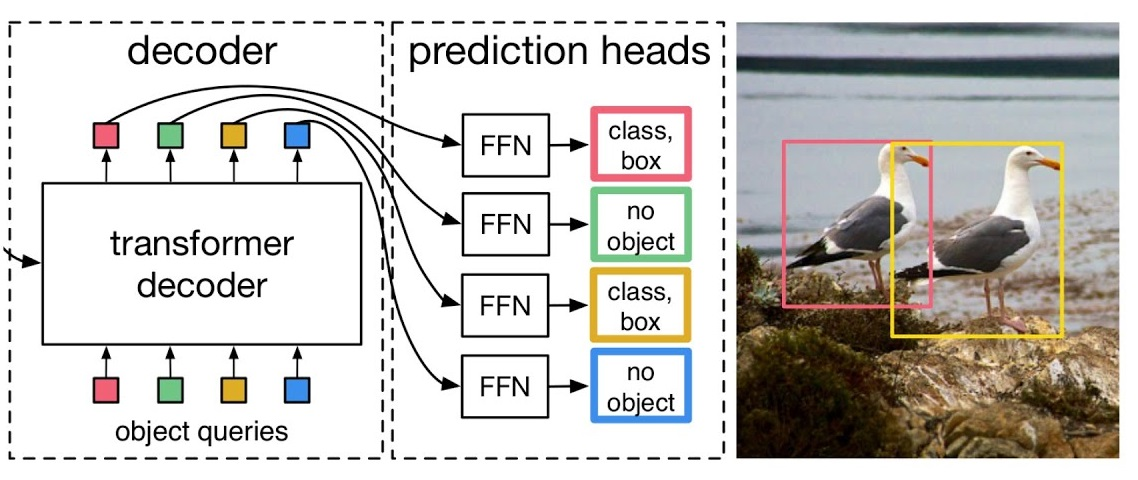
\includegraphics[width=0.85\linewidth]{data/detr}}
\caption{Схема сети DETR}
\label{detr_lbl}
\end{figure} 

Однако данный подход имеет ряд существенных недостатков:

1) самая важная проблема -- долгое и сложное обучение сети;

2) сеть DETR не является универсальной; существует ряд задач, в которых другие подходы проявляют себя значительно лучше 

\newpage
\subsection{Архитектура YOLO}
\newpage
\section{МОДЕЛИРОВАНИЕ НЕЙРОННОЙ СЕТИ}
\subsection{Описание используемого датасета}
Реализация задачи детекции в данной работе производилась на готовом датасете Car Object Detection, выгруженного с сайта, предлагающего готовые наборы данных для машинного обучения https://www.kaggle.com \cite{dataset}. Указанный набор содержит медиафайлы, снятые в условиях дорожной обстановки. На кадрах фиксировались автомобили. Исходные данные представляют собой два видеоряда, каждый из которых был разрезан на стоп-кадры (которые и являются исходными изображениями). Общее количество изображений в датасете равно 1001.  

Суть задачи сводится к тому, чтобы протестировать различные нейросетевые архитектуры, для обнаружения на изображении автомобилей. В датасете также имеются тренировочные изображения -- каждый автомобиль на них отмечен своей ограничивающей рамкой. 

Набор представляет собой изображения трех типов:

1) кадры, на которых имеется только один автомобиль;

2) кадры, на которых имеется несколько авиомобилей;

3) кадры, на которых нет автомобилей.

TO DO : Вставить изображения для каждого типа

Максимальное количество машин на изображении равно семи. Таким образом, задача усложняется тем, что исходное количество детектируемых на изображении объектов заранее неизвестно.
\newpage
\subsection{Предобработка датасета}

У трансформеров есть несколько ограничений при использовании. Одно из них связано с ограниченным фиксированным выходом из нейронной сети. Для того, чтобы избежать этой проблемы количество выходных объектов $K$ устанавливается значительно больше, чем максимальное ожидаемое количество объектов на изображениях. 

Для возможности сопоставления истинных меток с предсказанными нейронной сетью, датасет был преобразован способом, описанным ниже.
\begin{enumerate}
\item Координаты каждой ограничивающей рамки были преобразованы из абсолютных размеров, измеряемых в пикселях, в относительные по отношению к размерам изображения;
\item Полученные координаты переведены из описания левого верхнего угла $(x_{min}, y_{min})$ и правого нижнего $(x_{max}, y_{max})$ ограничивающей рамки в описание центра $(x_{c}, y_{c})$ и размеров изображения $(h, w)$;
\item Для каждого изображения все соответствующеи ему ограничивающие рамки были объединены в массив, который дополнили нулевыми ограничивающими рамками до размера массива равного $K$;
\item Каждой ограничивающей рамке была добавлена еще одна координата, соответствующая нахождению в ней объекта поиска, т.е. для ненулевых рамок 1, для остальных -- 0.
\end{enumerate}
Таким образом размерность метки для одного изображения равняется $(K, 5)$, при этом некоторые из рамок будут заполнены нулями.
\newpage
\subsection{Венгерский алгоритм}
\subsubsection*{Постановка задачи о назначениях}
Задача о назначениях -- это задача оптимизации, заключающаяся в поиске оптимального соответствия между двумя наборами элементов. В общем виде задача о назначениях формулируется следующим образом. 

Имеется $n$ работ и $n$ кандидатов для их выполнения. Затраты $i$ кандидата на выполнение $j$ работы равны $c_{ij}$. Каждый кандидат может быть назначен только на одну работу, и каждая работа может быть выполнена только одним кандидатом. Требуется найти назначение кандидатов на работы, при котором суммарные затраты на выполнение работ минимальны. 

Для построения математической модели вводятся переменные $x_{ij}$, принимающие значение 1 или 0 в зависимости от того, назначен или нет $i$ механизм на $j$ работу соответственно.

Тогда условие о том, что каждый кандидат выполняет только одну работу, запишется в виде 
\begin{equation}
\sum_{j=1}^{n} x_{ij} = 1, \quad \forall i = \overline{1,n}.
\end{equation}
Условие о том, что каждая работа может выполняться одним кандидатом, запишется в виде
\begin{equation}
\sum_{i=1}^{n} x_{ij} = 1, \quad \forall j = \overline{1,n}.
\end{equation}
Целевая функция примет вид
\begin{equation}
F = \sum_{i=1}^{n}\sum_{j=1}^{n} c_{ij} x_{ij}.
\end{equation}
В функцию войдут только те значения $c_{ij}$, для которых $x_{ij}$ отличны от 0, т.е. затраты, соответствующие назначенным работам.

В результате математическая модель задачи о назначениях принимает вид

\begin{equation}
  \left\{\begin{array}{l}
    k_{i\omega}/k_{p\omega}=2\pi\times 10\\
    \left|
      \frac{k_{p\omega}s+k_{i\omega}}{s}\cdot\frac{1}{Ts+1}
    \right|_{S=\mathrm{j}\cdot2\pi}=1
  \end{array}\right.\,.
\end{equation}



\newpage
\subsection{Функция потерь и сопоставление истинных и предсказанных меток}

В качестве функции потерь была выбрана следующая функция:
\begin{multline}
L \left(y_{true}, y_{pred}\right) = \lambda_1 BinCrossEntropy\left(p_{true}, p_{pred}\right) +\\
+\left\{p_{true}=1\right\} L_{bbox} \left(bbox_{true}, bbox_{pred}\right),
\end{multline}
где $y_{true} = (bbox_{true}, p_{true})$ -- истинная метка, $y_{pred} = (bbox_{pred}, p_{pred})$ -- метка, предсказанная нейросетью, $bbox_{true}, bbox_{pred}$ -- ограничивающие рамки объекта, $p_{true}, p_{pred}$ -- вероятность нахождения объекта в ограничивающей рамке, $\lambda_1$ -- гиперпараметр. 

Функции $BinCrossEntropy\left(p_{true}, p_{pred}\right)$ и $L_{bbox} \left(bbox_{true}, bbox_{pred}\right)$ определяются следующим образом:
\begin{multline}
BinCrossEntropy\left(p_{true}, p_{pred}\right) = - p_{true} \log(p_{pred}) -\\ - ( 1 - p_{true} ) \log(1 - p_{pred}),
\end{multline}
\begin{multline}
L_{bbox} \left(bbox_{true}, bbox_{pred}\right) = - \lambda_2 \log(IoU\left(bbox_{true}, bbox_{pred}\right)) +\\ + \lambda_3 \parallel bbox_{true} - bbox_{pred}\parallel_1,
\end{multline}
где $\lambda_2$, $\lambda_3$ -- гиперпараметры, $\parallel \cdot \parallel_1$ -- L1 норма.

IoU (Intersection over Union) -- площадь пересечения ограничивающих рамок, деленная на площадь их объединения.
\begin{figure}[h]
\center{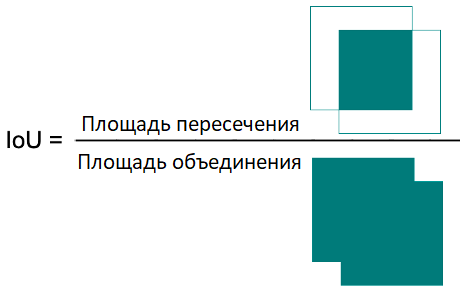
\includegraphics[width=0.6\linewidth]{data/IoU.png}}
\caption{IoU}
\label{IoU}
\end{figure}  


Для того чтобы определить соответствие между объектами на входном и выходном изображениях, используется венгерский алгоритм. Он находит наилучшее соответствие между объектами таким образом, чтобы минимизировать общую ошибку.
Его использование реализовано следующим образом:
\begin{enumerate}
\item Для каждого $y_{true}$ и $y_{pred}$ вычисляется значение функции потерь $L$;
\item На полученной матрице $C$ размера $(K,K)$, используется венгерский алгоритм.
\end{enumerate}

\newpage
\subsection{Используемые метрики}
Тут про IoU с венгреским алгоритмом и так же про вероятности (Hang\_p).

\newpage
\subsection{Используемые слои и структуры}
\subsubsection*{Полносвязный слой}
Полносвязные слои (Fully Connected или Dense layers) - это тип слоев в нейронных сетях, который применяет линейную функцию к каждому входному элементу (нейрону) и создает новые признаки с заданной размерностью.

Пусть вход в слой имеет размерность (N, M), где N - это количество примеров (например, изображений), а M - это размерность каждого примера (например, количество пикселей в изображении). Полносвязный слой преобразовывает каждый пример размерности (1, M) в новый пример размерности (1, K), где K - это заданное число новых признаков. Этот процесс происходит путем умножения входа на матрицу весов размерности (M, K), после чего к результату прибавляется вектор смещения размерности (1, K). В общем случае, формула для вычисления выхода из полносвязного слоя будет выглядеть следующим образом:
$$y = Wx + b,$$
где $x$ -- входной тензор, $W$ -- матрица весов, $b$ -- вектор смещения, а $y$ -- вы\-ход\-ной тензор.

После вычисления выхода из полносвязного слоя, к результату может быть применена некоторая нелинейная функция активации, такая как ReLU, Sigmoid, Tanh и другие. Нелинейная функция активации обычно используется для того, чтобы преобразовать выход полносвязного слоя в нелинейный диапазон значений и добавить нелинейность в модель, что может улучшить ее способность обобщения и улучшить качество предсказаний.

\subsubsection*{Слой Dropout}
Слой Dropout - это техника регуляризации, которая используется в нейронных сетях для предотвращения переобучения. Идея Dropout заключается в том, чтобы случайно удалять (выключать) некоторые нейроны в каждом слое, во время обучения сети.

Каждый нейрон в слое Dropout имеет вероятность p (обычно 0.5) быть выключенным в каждом проходе обучения. При этом, выходы всех нейронов будут умножены на 1/(1-p), чтобы уравнять суммарную величину выходных данных слоя.

Таким образом, когда происходит проход обучения сети, Dropout выключает случайно выбранные нейроны в каждом проходе. Это заставляет нейроны в слое работать более самостоятельно, а не перенаправляться на зависимости, которые могут быть связаны с конкретными нейронами. Dropout также заставляет сеть учитывать более разнообразное представление входных данных, что обычно приводит к улучшению обобщающей способности модели.

После обучения, Dropout отключается, и все нейроны начинают работать с соответствующими весами. В этом случае, устанавливается режим "inference" (применения), и каждый нейрон является активным.

Слой Dropout часто используется вместе с полносвязными слоями (Dense layers) или сверточными слоями (Convolutional layers) в глубоких нейронных сетях, особенно в случае, когда обучение сети сталкивается с проблемой переобучения. Dropout позволяет контролировать сложность модели, предотвращает переобучение и улучшает ее обобщающую способность.


\subsubsection*{Слой Patches}
В реализации сети Transformer с архитектурой ViT каждое изображение делится на патчи. Для этого создается специальный слой Patches. На вход данный класс будет принимать только размеры самих патчей. При его вызове в него передается всё входное изображение. Далее это изображение будет разделено на патчи указанного размера и каждый из них будет вытянут в одномерный вектор признаков.


\subsubsection*{Слой PatchEncoder}
Для каждого из патчей важно помнить правильное их расположение. Поэтому в сети используется слой PatchEncoder. На вход данный класс будет принимать количество патчей изображения и размерность обучаемых эмбедингов. Эти эмбединги необходимы для кодирования номера патча в разделенном изображении. Каждый патч проходит через полносвязный слой с количеством выходов равным размерности эмбедингов. К полученному результату прибавляется значение эмбединга соответствующее номеру патча в изображении. Таким образом на выходе слоя PatchEncoder будет вектор с размерностью эмбедингов для каждого патча.

\subsubsection*{Слой LayerNormalization}
LayerNormalization

\newpage
\subsection{Реализация сети ViT}
Реализовано на языке Python.
Основные используемые пакеты Tensorflow и в частности его модуль Keras.

Потом описываем функцию построения модели: сначала входной слой такой-то, который подается на такие-то слои и далее
Какие-то слои повторяются несколько раз, меняя только кол-во фильтров

\newpage
\subsection{Предобработка датасета для сети YOLO}

\newpage
\section{РЕЗУЛЬТАТЫ МОДЕЛИРОВАНИЯ}
\subsection{Сеть ViT}

В качестве архитектуры сети была выбрана архитектрура ViT.
Для проверки качества обучения сети использовались следующие метрики
\begin{enumerate}
\item Средний IoU (Intersection over Union) -- Среднее арифметическое отношений пересечения площадей ограничивающих рамок и их объединения;
\item Точность -- отношение количества правильно меток присутствия объекта к количеству всех предсказаний.
\end{enumerate}

Обучение сети проводилось 800 эпох. Наилучшие достигнутое значение среднего IoU равняется 54.5\%. Для точности  -- 98.4\%. Результаты обучения сети представлены на рис. \ref{mIoU} и рис. \ref{Acc}.
\begin{figure}[h!]
\center{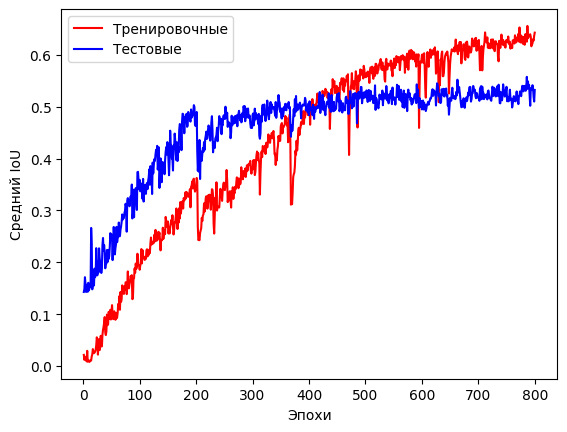
\includegraphics[width=1.\linewidth, height=0.55
\textheight]{data/mean_IoU}}
\caption{График среднего IoU алгоритма ViT}
\label{mIoU}
\end{figure} 

Скачки, представленные на графиках, могут быть вызваны за счет использования венгерского алгоритма: поскольку у сети 10 разных выходов, каждый из которых обучается отдельно, в следствие чего в процессе обучения венгерский алгоритм возвращает разные перестановки выходов.

\begin{figure}[h!]
\center{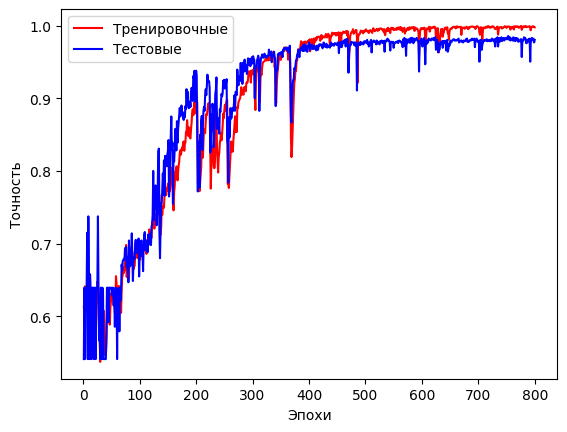
\includegraphics[width=1.\linewidth, height=0.55
\textheight]{data/Accuracy}}
\caption{График точности алгоритма ViT}
\label{Acc}
\end{figure} 

Ниже на рис. \ref{result1} и рис. \ref{result4} представлены примеры обнаружения автомобилей с помощью нейронной сети и сравнение предсказанных ограничивающих рамок с истинными.

\newpage
\begin{figure}[h!]
\center{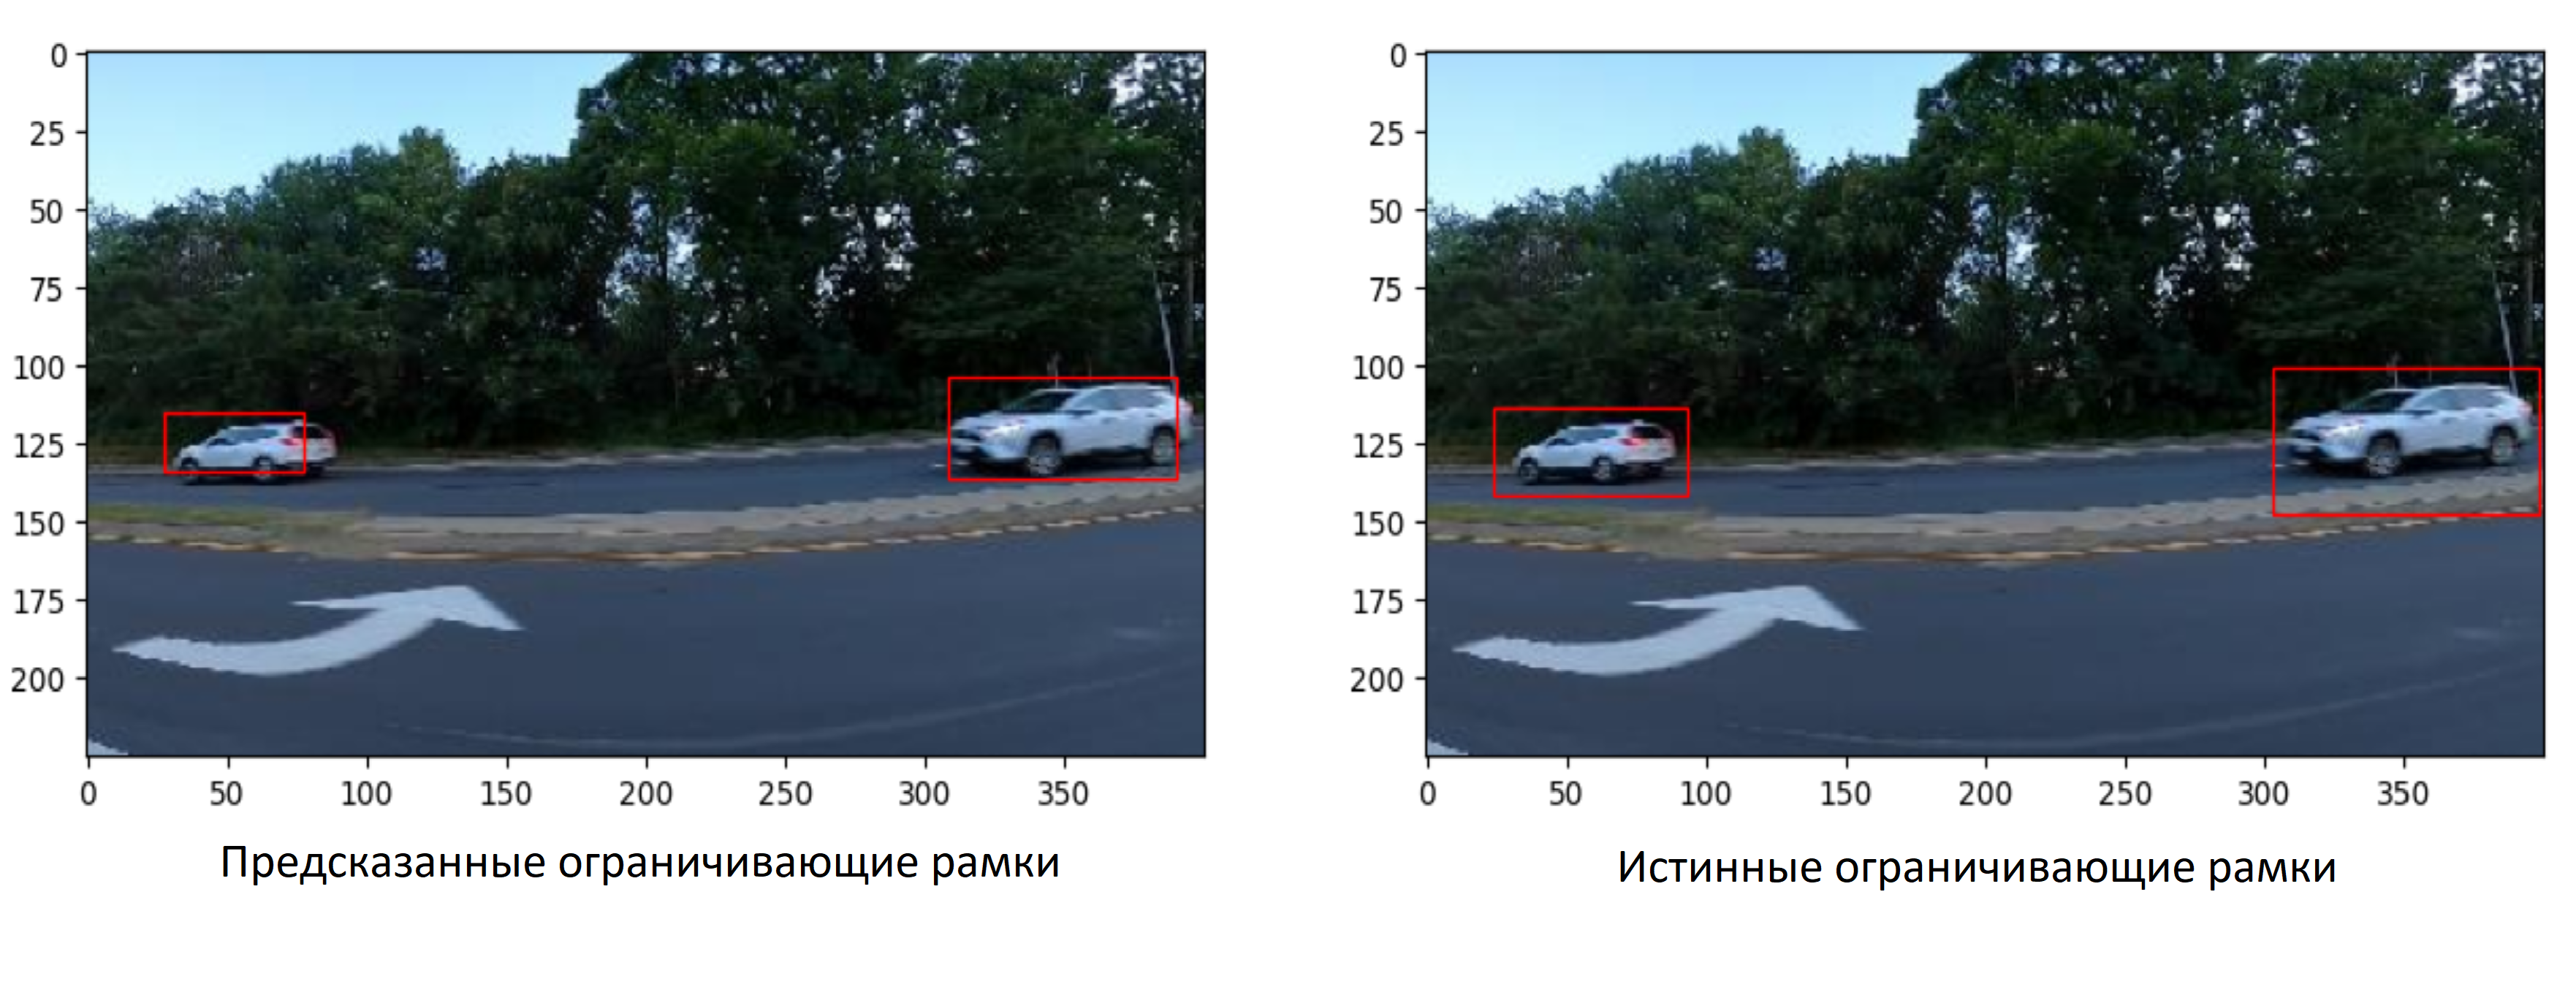
\includegraphics[width=1\linewidth]{data/result1}}
\caption{Первый пример обнаружения объектов ViT нейросетью}
\label{result1}
\end{figure} 

\begin{figure}[h!]
\center{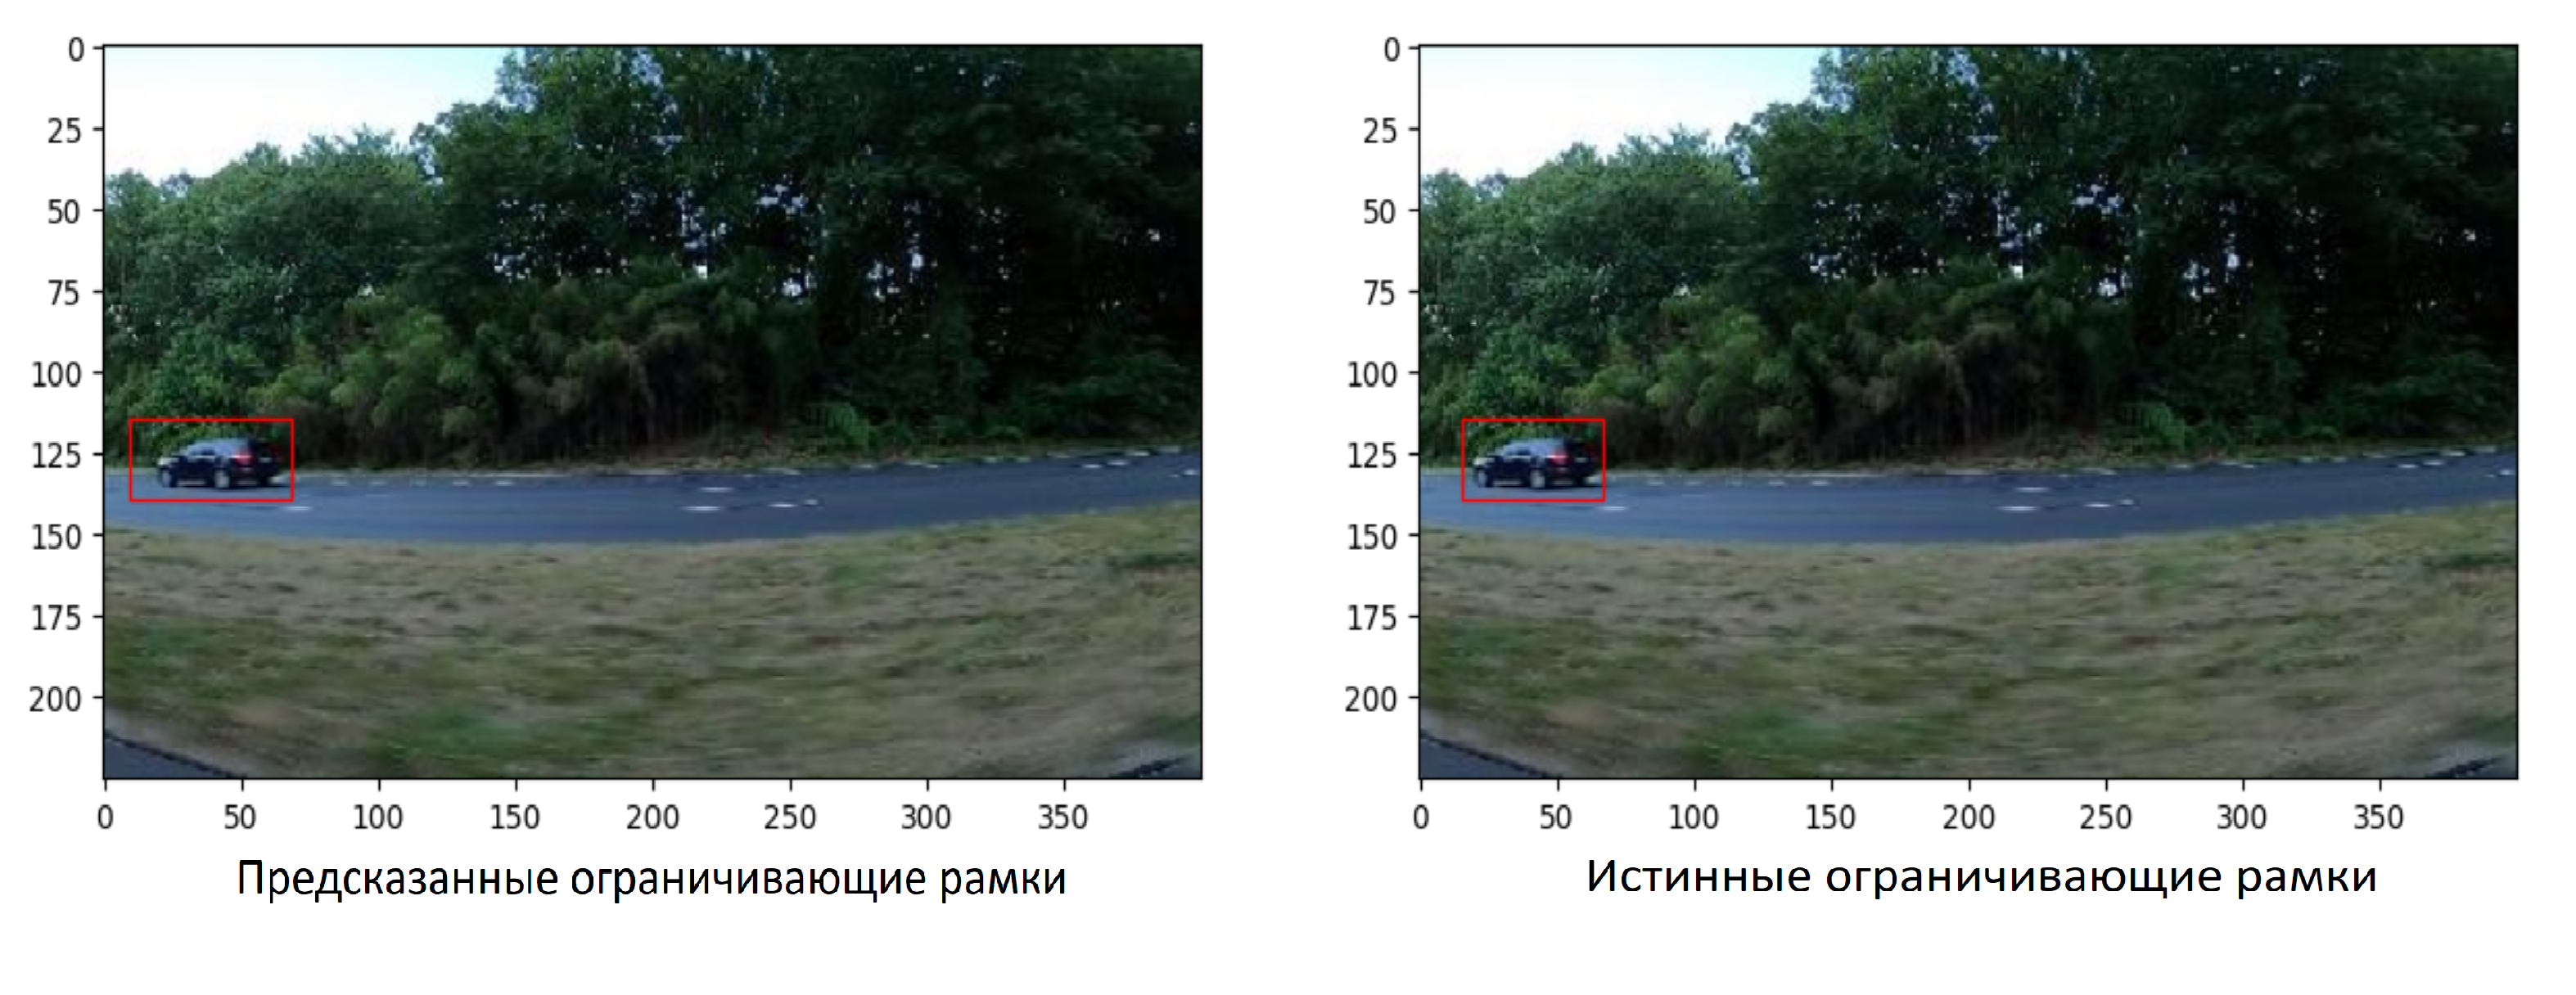
\includegraphics[width=1\linewidth]{data/result4}}
\caption{Второй пример обнаружения объектов ViT нейросетью}
\label{result4}
\end{figure} 

\newpage
\subsection{Сеть YOLO}

\newpage
\section-{ЗАКЛЮЧЕНИЕ}

В настоящей работе было дано определение задаче обнаружения объектов, позволяющая выделять и классифицировать объекты на изображении.
Рассмотрена нейросетевая архитектура Transformer, разобраны основные составляющие. Описан механизм внимания, способ его вычисления. Исследован слой Multi-head attention, а так же его связь с механизмом внимания. Рассмотрены 2 нейронных сети с использованием Transformer: Vit и DETR, их основные особенности и различия.

Реализована и протестирована нейросеть ViT. Были представлены графики, полученные в результате обучения.


\newpage
\begin{thebibliography}{99}
\bibitem{cnn} Муаль М.Н.Б., Козырев Д.В., Уанкпо Г.Ж.К., Нибасумба Э. Разработка нейросетевого метода в задаче классификации и распозна-
вании изображения // Современные информационные технологии и ИТ-образование. ‒
2021. ‒ Т. 17, № 3. – С. 507-518.

\bibitem{cod_decod} Kyunghyun Cho, Bart van Merrienboer, Caglar Gulcehre, Dzmitry Bahdanau, Fethi Bougares, Holger Schwenk, Yoshua Bengio. Learning Phrase Representations using RNN Encoder-Decoder for Statistical Machine Translation [Электронный ресурс] // ArXiv : [сайт]. — URL: https://arxiv.org/abs/1406.1078 (дата обращения: 28.05.2023).

\bibitem{transform} Ashish Vaswani, Noam Shazeer, Niki Parmar, Jakob Uszkoreit, Llion Jones, Aidan N. Gomez, Lukasz Kaiser, Illia Polosukhin. Attention Is All You Need [Электронный ресурс] // arXiv : [сайт]. — URL: https://arxiv.org/pdf/1706.03762.pdf (дата обращения: 26.05.2023).

%\bibitem{vvedenie1} https://www.mathnet.ru/links/f82cbf8ad152bf35475641dfea9ea63e/ps397.pdf
\bibitem{dataset} EDWARD ZHANG. Car Object Detection [Электронный ресурс] // Kaggle : [сайт]. — URL: https://www.kaggle.com/datasets/sshikamaru/car-object-detection (дата обращения: 26.05.2023).

\end{thebibliography}

\end{document} 